% Created 2024-10-07 Mon 07:06
% Intended LaTeX compiler: pdflatex
\documentclass[11pt]{article}
\usepackage[utf8]{inputenc}
\usepackage[T1]{fontenc}
\usepackage{graphicx}
\usepackage{longtable}
\usepackage{wrapfig}
\usepackage{rotating}
\usepackage[normalem]{ulem}
\usepackage{amsmath}
\usepackage{amssymb}
\usepackage{capt-of}
\usepackage{hyperref}
\date{\today}
\title{Org-mode PDF}
\begin{document}

\maketitle
\tableofcontents

\#+latex\textsubscript{header}

\section{Red borders around PDF ToC elements}
\label{sec:org1169bd8}

\begin{center}
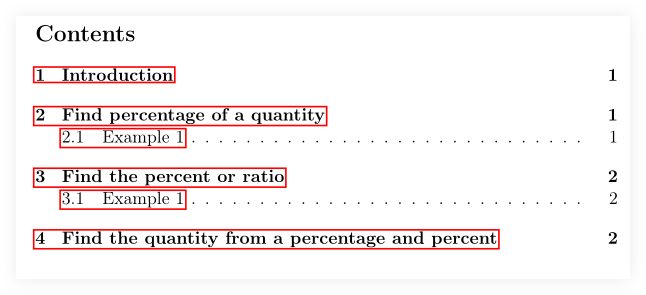
\includegraphics[width=.9\linewidth]{__assets/org_20241006-084242_org-pdf-uggly-red-borders-on-toc.png}
\end{center}

One solution is to do it on a per buffer basis:

\begin{verbatim}
#+latex_header: \hypersetup{colorlinks=true,linkcolor=black}
\end{verbatim}

\subsection{References}
\label{sec:orgfec15f8}

\begin{itemize}
\item \href{https://emacs.stackexchange.com/questions/29640/how-do-i-get-rid-of-the-red-boxes-around-the-links-in-the-toc}{How do I get rid of the red boxes around the links in the TOC?
(Emacs on Stack Exchange)}.
\item \href{https://emacs.stackexchange.com/questions/12878/how-to-change-style-of-hyperlinks-within-pdf-published-from-org-mode-document}{How to change style of hyperlinks within PDF published from org-mode document? (Emacs on Stack Exchange)}.
\end{itemize}
\end{document}
